\begin{figure}[!ht]
	\centering
	\setlength{\resLen}{1.in}
	\setlength{\raiseLen}{0.4in}
	\addtolength{\tabcolsep}{-4pt}
	\begin{tabular}{cccc}
		& SVBRDF maps & Optimization & Novel
		\\
		\raisebox{\raiseLen}{\rotatebox[origin=c]{90}{GT}} &
		\includegraphics[height=\resLen]{svbrdf/validation/noise_refine/fake_037/ref/tex.jpg} &
		
\includegraphics[height=\resLen]{svbrdf/validation/noise_refine/fake_037/ref/00.jpg} &
		
\includegraphics[height=\resLen]{svbrdf/validation/noise_refine/fake_037/ref/07.jpg}
		\\
		\raisebox{\raiseLen}{\rotatebox[origin=c]{0}{(1)}} &
		\includegraphics[height=\resLen]{svbrdf/validation/noise_refine/fake_037/optimW+N/tex.jpg} &
		
\includegraphics[height=\resLen]{svbrdf/validation/noise_refine/fake_037/optimW+N/00.jpg} &
		
\includegraphics[height=\resLen]{svbrdf/validation/noise_refine/fake_037/optimW+N/07.jpg}
		\\
		\raisebox{\raiseLen}{\rotatebox[origin=c]{0}{(2)}} &
		\includegraphics[height=\resLen]{svbrdf/validation/noise_refine/fake_037/optimW+_refine/tex.jpg} &
		
\includegraphics[height=\resLen]{svbrdf/validation/noise_refine/fake_037/optimW+_refine/00.jpg} &
		
\includegraphics[height=\resLen]{svbrdf/validation/noise_refine/fake_037/optimW+_refine/07.jpg}
		\\
		\raisebox{\raiseLen}{\rotatebox[origin=c]{90}{GT}} &
		 &
		
\includegraphics[height=\resLen]{svbrdf/validation/noise_refine/real_book1/ref/00.jpg} &
		
\includegraphics[height=\resLen]{svbrdf/validation/noise_refine/real_book1/ref/07.jpg}
		\\
		\raisebox{\raiseLen}{\rotatebox[origin=c]{0}{(1)}} &
		\includegraphics[height=\resLen]{svbrdf/validation/noise_refine/real_book1/optimW+N/tex.jpg} &
		
\includegraphics[height=\resLen]{svbrdf/validation/noise_refine/real_book1/optimW+N/00.jpg} &
		
\includegraphics[height=\resLen]{svbrdf/validation/noise_refine/real_book1/optimW+N/07.jpg}
		\\
		\raisebox{\raiseLen}{\rotatebox[origin=c]{0}{(2)}} &
		\includegraphics[height=\resLen]{svbrdf/validation/noise_refine/real_book1/optimW+_refine/tex.jpg} &
		
\includegraphics[height=\resLen]{svbrdf/validation/noise_refine/real_book1/optimW+_refine/00.jpg} &
		
\includegraphics[height=\resLen]{svbrdf/validation/noise_refine/real_book1/optimW+_refine/07.jpg}
	\end{tabular}
	\caption[Noise optimization vs. post-refinement]{\label{fig:svbrdf:noise_vs_refine}
		\textbf{Noise optimization vs. post-refinement.} (1) Optimize $\bmw^+$ and $\bmxi$ but no post-refinement; (2) Optimize $\bmw^+$ only but with post-refinement. This shows that $\bmxi$ takes an important role; optimizing only $\bmw^+$ has too little expressive power and converges to suboptimal solutions, which post-refinement cannot fix (see especially normal maps in (2)).
	}
\end{figure}